% A rough draft of the proof of the simple instruction reordering, given the memory model



\section{Instruction Reordering}
    Instruction reordering is a common operation in compiler optimization, essential to instruction scheduling of course, but also implicit in loop invariant removal, partial redundancy elimination, and other optimizations that may move instructions. 
    However, whether we can do such reordering freely given a concurrent program using relaxed memory accesses is a bit unclear. 
     
    
    \paragraph{Simple reordering is not straightforward under shared memory semantics}
    The main reason is that memory accesses here, do not just perform the desired operation (i.e Read / Write) but also imply certain visibility guarantees across all the other threads.  
    In our observation, we find that, the relaxed memory model of Javascript prescribe semantics for visibility using the $\stck{_{hb}}$ relations. 
    
    \critic{purple}{Show an example or multiple examples here that enforces visibility due to having sequentially consistent events involved in a Candidate Execution.}
    
    \paragraph{What can be done?}
    An example-based analysis exposes to us the problems that might exist when we perform such reordering of events. 
    However, such an analysis, though would work for small programs to identify the possible conditions under which reordering can be done, become infeasible as the programs scale in length and complexity. 
    This is because of the exponential increase in possible executions as the number of threads and program size in general increase. 
    Hence,  generalizations by using a small sample size is not something we can afford especially when we want to ensure these program trasnformations are done by the compiler in contrast to being done manually.
    
    \paragraph{Our approach}
    Our solution to this is to construct a proof on Candidate Executions of the original program and the transformed one which exposes the possible observable behaviors it can have.   
    The crux of the proof is to guarantee that reordering does not bring any new $\stck{_{rf}}$ (reads-from) relations that did not exist in any Observable Behavior of the original Candidate Execution. 
    It is important to note however, that a proof in this sense would be generalized to any Candidate and is thus conservative.
    So, it might be the case that for specific programs, reordering can be valid, however, in a general sense may not be valid for others. 

    \paragraph{Assumption}
    We make the following assumptions for every program we consider :
    \begin{enumerate}
        \item All events are tear-free
        \item No synchronize events exist
        \item No Read-Modify-Write events exist
        \item All executions of the candidate before reordering have happens-before as a strict partial order
    \end{enumerate}
    
    We first consider when consecutive events in the same agent can be reordered, followed by non-consecutive cases. The crux of the proof is to guarantee that reordering does not bring any new reads-from relations that did not result due to any execution of the original program. 
    
    %GIVE TWO EXAMPLES TO SHOW THIS. POSSIBLY USE THE EXAMPLE ABOVE AND EXPLAIN

        \subsection{Preliminaries}
    Before we go about proving when reordering is valid, we would like to have two additional definitions which would prove useful.
    
    %Something we need to define for sake of proofs
    \begin{definition}{Consecutive pair of events (\emph{cons})}
        
        We define \emph{cons} as a function, which takes two events as input, and gives us a boolean indicating if they are consecutive pairs. Two events $e$ and $d$ are consecutive if they have an $\stck{_\textit{ao}}$ relation among them and are \emph{next to each other} in the same agent (thread), which can be defined formally as 
            \begin{align*}
                (
                e \stck{_\textit{ao}} d  \ \wedge \ 
                \nexists k \ \textit{s.t.} \ 
                e \stck{_\textit{ao}} k  \ \wedge \
                k \stck{_\textit{ao}} d 
                )
                \ \vee \
                (
                    d \stck{_\textit{ao}} e  \ \wedge \ 
                    \nexists k \ \textit{s.t.} \ 
                    d \stck{_\textit{ao}} k  \ \wedge \
                    k \stck{_\textit{ao}} e  
                )
            \end{align*}
    \end{definition}

    \begin{definition}{Direct happens-before relation (dir)}
        
        We define \emph{dir} to take an ordered pair of events $(e,d)$ such that $\reln{e}{hb}{d}$ and gives a boolean value to indicate whether this relation is \textit{direct}, i.e those relations that are not derived through transitive property of $\stck{_\textit{hb}}$.

        %Perhaps put a formal defintion here 
        
        We can infer certain relations/conditions that must hold using this function based on some information on events $e$ and $d$. 
        \begin{itemize}
            \item If $\et{e}{uo}$, then $dir(e,d) \ \Rightarrow \ cons(e,d)$
            \item If $\et{d}{uo}$, then $dir(e,d) \ \Rightarrow \ cons(e,d)$
            \item If $\et{e}{sc}\ \wedge\ e\!\in\!R$, then $dir(e,d) \ \Rightarrow \ cons(e,d)$
            \item If $\et{e}{sc}\ \wedge\ e\!\in\!W$, then $dir(e,d) \ \Rightarrow \ cons(e,d)\ \vee\ \reln{e}{sw}{d}$
            \item If $\et{d}{sc}\ \wedge\ d\!\in\!W$, then $dir(e,d) \ \Rightarrow \ cons(e,d)$
            \item If $\et{d}{sc}\ \wedge\ e\!\in\!R$, then $dir(e,d) \ \Rightarrow \ cons(e,d)\ \vee\ \reln{e}{sw}{d}$
        \end{itemize}
    \end{definition}


    \subsection{Lemmas to assist our proof}    
In order to assist our proof, we define two \textit{lemmas} based on the ordering relations. 

\begin{lemma} Consider three events $e$,$d$ and $k$. \\

    If
        \[
            \cons{e}{d} \ \wedge \ \reln{e}{ao}{d} \ \wedge \
            (
                (\et{d}{uo}) \ \vee \
                (\et{d}{sc} \ \wedge \ \event{d}{W})
            )
        \]
        
    then,
        \[
            \reln{k}{hb}{d} \Longrightarrow \reln{k}{hb}{e}
        \]
      
    When we have two consecutive events \textit{e} and \textit{d} which are one after the other (i.e. $\reln{e}{ao}{d}$), we can use \textit{transitive property} of $\stck{_{hb}}$ to infer that any event \textit{k} that \textit{happens before} \textit{e}, also \textit{happens before} \textit{d}. However, is it possible to derive that the event \textit{k happens before e} using the evidence that \textit{k happens before d} ? This lemma states the condition when this is true.
    
\end{lemma}

%An alternative short proof 
\begin{proof}
    
    We will divide the proof for this into two cases, based on what event $d$ is. For both cases, we have the following to be true :
    
    \[
        cons(e,d) \ \wedge \ \reln{e}{ao}{d}
        \tag{0}
        \label{l10}
    \]

    In the first case, 
    
    \[
        \et{d}{uo} 
        \tag{1}
        \label{l11}
    \]
    
    Then for any event $k$
    \[
        dir(k,d) \Rightarrow cons(k,d)
        \qquad from \quad
        (\ref{l11})
        \tag{2}
        \label{l12}
    \]
    
    An event that satisfies the above with $d$ is $e$.
    \[
         k = e  
         \qquad from \quad
         (\ref{l10}, \ref{l12})
         \tag{3}
         \label{l13}
    \]
    
    Because $\stck{_{ao}}$ is a total order, $e$ will be the only event. This would mean that for any other $k \neq e$,
    
    \[
        \reln{k}{hb}{d} \Rightarrow \reln{k}{hb}{d}
        \qquad from \quad
        (\ref{l10}, \ref{l11}, \ref{l12}, \ref{l13}) 
    \]
    
    The following figure should explain this intuition:  
    \begin{figure}[H]
        \centering
        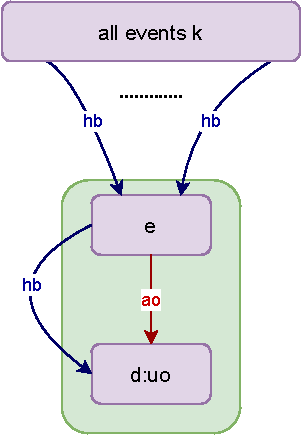
\includegraphics[scale=0.7]{InstructionReordering/Lemmas/lemma_proof1_case1.pdf}
        \caption{For the first case}
        \label{fig:my_label}
    \end{figure}
    
    In the second case,
    \[
        \et{d}{sc} \wedge d\!\in\!W
        \tag{4}
        \label{l14}
    \]
    
    Then for any event $k$
    \[
        dir(k,d) \Rightarrow cons(k,d)
        \qquad from \quad
        (\ref{l14})
        \tag{5}
        \label{l15}
    \]
    
    We once again have event $e$ satisfying the above
    \[
        k = e 
        \qquad from \quad
        (\ref{l10}, \ref{l15})
        \tag{6}
        \label{l16}
    \]
    
    Though there could be direct \textit{happens-before} relation with some event $k$ from another \textit{agent}, these are only relations satisfying $dir(d,k)$. Thus, we can once again infer that for any $k \neq e$ 
    
    \[
        \reln{k}{hb}{d} \Rightarrow \reln{k}{hb}{d}
        \qquad from \quad
        (\ref{l10}, \ref{l14}, \ref{l15}, \ref{l16})
    \]
    
    The following figure explains this intuition: 
    
    \begin{figure}[H]
        \centering
        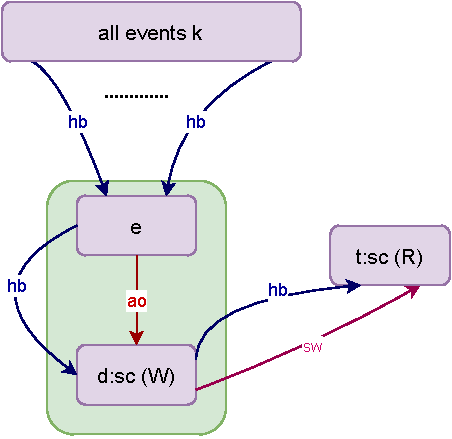
\includegraphics[scale=0.7]{InstructionReordering/Lemmas/lemma_proof1_case2.pdf}
        \caption{For the second case}
        \label{fig:my_label}
    \end{figure}
    
\end{proof}

%---------------------------------------------------------------------------------------------------------------    

%SHORTER VERSION OF PROOF WITHOUT THE ENGLISH EXPLAINATION IN THE MIDDLE. DISCUSS AND DECIDE ON WHICH FORM IS BETTER
\begin{lemma}Consider three events $e$, $d$ and $k$ \\

    If
        
        \[
            \cons{e}{d} \ \wedge \ \reln{e}{ao}{d} \ \wedge \
            (
                (\et{e}{uo}) \ \vee \
                (\et{e}{sc} \ \wedge \ \event{e}{R})
            )
        \]
        
    then,
        \[
            \reln{e}{hb}{k} \Longrightarrow \reln{d}{hb}{k}
        \]

 When we have two consecutive events \textit{e} and \textit{d} which are one after the other (i.e. $\reln{e}{ao}{d}$), we can use \textit{transitive property} of $\stck{_{hb}}$ to infer that any event \textit{k} that \textit{happens after} \textit{d}, also \textit{happens after} \textit{e}. However, is it possible to derive that the event \textit{k happens after d} using the evidence that \textit{k happens after e} ? This lemma states the condition when this is true.

\end{lemma}

%An alternative proof for this 
\begin{proof}
    
    Just like the proof for the previous lemma, we will divide the proof for this into two cases, based on what event $e$ is. Again, for both cases, we have the following to be true:
    
    \[
        cons(e,d) \ \wedge \reln{e}{ao}{d}
        \tag{0}
        \label{l20}
    \]

   In the first case,
   
   \[
        \et{e}{uo} 
        \tag{1}
        \label{l21}
   \]
   
   Then for any event k
   
   \[
        dir(e,k) \Rightarrow cons(e,k) 
        \qquad from
        \quad (\ref{l21})
        \tag{2}
        \label{l22}
   \]
   
   The event that satisfies the above with $e$ is $d$
   \[
        k = d 
        \qquad from 
        \quad (\ref{l20}, \ref{l22})
        \tag{3}
        \label{l23}
   \]
   
   Because $\stck{_{ao}}$ is a total order, $d$ would be the only such event. This would mean that for any other event $k \neq d$
   
   \[
        \reln{e}{hb}{k} \Rightarrow \reln{d}{hb}{k}
        \qquad from 
        \quad (\ref{l20}, \ref{l21}, \ref{l22}, \ref{l23})
   \]
   %Better phrase the intuition
   The following figure should explain this intuition:  
    
    \begin{figure}[H]
        \centering
        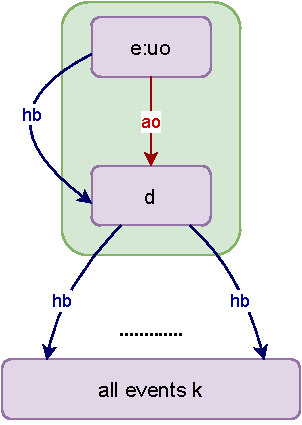
\includegraphics[scale=0.7]{InstructionReordering/Lemmas/lemma_proof2_case1.pdf}
        \caption{Caption}
        \label{fig:my_label}
    \end{figure}
    
    In the second case,
    \[
        \et{e}{sc} \wedge e\!\in\!R
        \tag{4}
        \label{l24}
    \]
    
    Then for any event $k$
    \[
        dir(e,k) \Rightarrow cons(e,k)
        \qquad from \quad
        (\ref{l24})
        \tag{5}
        \label{l25}
    \]
    
    We once again have event $d$ satisfying the above   
    \[
        k = d 
        \qquad from \quad
        (\ref{l20}, \ref{l25})
        \tag{6}
        \label{l26}
    \]
    
    Though there could be direct \textit{happens-before} relation with some event $k$ from another \textit{agent}, these are only relations satisfying $dir(k,e)$. Thus, we can once again infer that for any $k \neq d$ 
    
    \[
        \reln{e}{hb}{k} \Rightarrow \reln{d}{hb}{k}
        \qquad from \quad
        (\ref{l10}, \ref{l24},  \ref{l25}, \ref{l16})
    \]
    
    The following figure explains this intuition: 
    
    \begin{figure}[H]
        \centering
        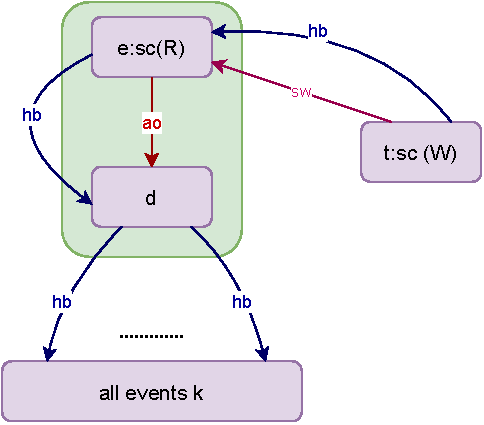
\includegraphics[scale=0.7]{InstructionReordering/Lemmas/lemma_proof2_case2.pdf}
        \caption{Caption}
        \label{fig:my_label}
    \end{figure}

\end{proof}

%------------------------------------------------------------------------------


\subsection{Valid reordering}
    We view reordering as manipulating the agent-order relation among two events. In that sense, reordering two consecutive events $e$ and $d$ such that $e \stck{_{ao}} d$ becomes:
    \[
        e \stck{_{ao}} d 
        \longmapsto
        d \stck{_{ao}} e 
    \]

    What implications this change has on the other ordering relations depends on the type of events $e$ and $d$ are and would require an analysis on each Candidate Execution. 
    The intuition is that the axioms of the memory model rely on certain ordering relations to restrict observable behaviors in a program.
    Hence, preserving these ordering relations would help us in turn not introduce new Observable Behaviors.
    In particular we note that preserving $\stck{_{hb}}$ relations (other than the one we eliminate intentionally i.e $\reln{e}{hb}{d}$) would suffice for our purpose. 
    Since $\stck{_{mo}}$ respects $\stck{_{hb}}$, we in turn even preserve the memory order which is essential.  

    In the end, we want to ensure that the set of possible observable behaviors of a program, remain unchanged after reordering. If that is not feasible, then we would want the set of observable behaviors after reordering at the very least to be a subset. This would ensure that the program does not have some new behaviours that weren't supposed to happen prior to reordering. 
    
    We begin by first defining a reorderable pair of events. We then formulate a theorem (with a proof) on the set of observable behaviors of a Candidate before and after reordering a pair of consecutive events which are reorderable. We consider reordering valid if the set of observable behaviours after reordering are a subset of the original. 

    \begin{definition}{Reorderable Pair (Reord)}
        We define a boolean function \emph{Reord} that takes two ordered pair of events $e$ and $d$ such that $\reln{e}{ao}{d}$ and gives a boolean value indicating if they are a reorderable pair. 
        
        \begin{align*}
            Reord(e,d) = \\
            (
            &((\et{e}{uo} \ \wedge \ \et{d}{uo}) \ \wedge \ 
                    (   
                        (\event{e}{R} \ \wedge \ \event{d}{R}) \ \vee \ 
                        (\Re(e) \cap_\Re \Re(d) = \phi) 
                    )
            ) \\ &\vee \\
            &((\et{e}{sc} \ \wedge \ \et{d}{uo}) \ \wedge \ 
                    (
                        (\event{e}{W} \ \wedge \ (\Re(e) \cap_\Re \Re(d) = \phi)) 
                    )
            ) \\ &\vee \\
            &((\et{e}{uo} \ \wedge \ \et{d}{sc}) \ \wedge \ 
                    (
                        (\event{d}{R} \ \wedge \ (\Re(e) \cap_\Re \Re(d) = \phi)) 
                    )
            )
            )
        \end{align*}

        \critic{purple}{Use the latter for the purpose at the end of the proof for reordering, to emphasize how we approached each case}

         
    \end{definition}

\begin{theorem} 

    Consider a candidate $C$ of a program and its possible \textit{Candidate Executions} where $\stck{_\textit{hb}}$ is strictly partial order. Consider two events $e$ and $d$ such that $\cons{e}{d}$ is true in $C$ and  $\reln{e}{ao}{d}$. Consider another candidate $C'$ resulting after reordering $e$ and $d$. 
    Then if \emph{Reord(e,d)} is true in $C$, the set observable behaviors possible due to Candidate Executions of $C'$ is a subset of that of $C$. 
\end{theorem}

\begin{proof}

    We look at this in terms of performing an instruction reordering on a candidate execution of $C$. We would want the resulting candidate execution to preserve all the other $\stck{_{hb}}$ relations (except $\reln{e}{hb}{d}$) and that any new $\stck{_{hb}}$ relations strictly reduce possible observable behaviors.
    
    The proof is structured as follows. We first show that existing \textit{happens-before} relations in any candidate execution of $C$ except $\reln{e}{hb}{d}$ remain intact after reordering. We then identify the cases where new \textit{happens-before} relations could be established. We identify from these cases whether \textit{happens-before} cycles could be introduced.
    We then show for the remaining cases that new relations do not introduce any new observable behaviors.

    The above steps can be summarized as addressing four main questions for any $Candidate Execution$ of $C'$
    \begin{enumerate}
        \item Apart from $\reln{e}{hb}{d}$, do other \emph{happens-before} relations remain intact?
        \item Apart from $\reln{d}{hb}{e}$, are any new \emph{happens-before} relations established? 
        \item Are any \emph{happens-before} cycles introduced? 
        \item Do the new relations bring new \emph{observable behaviors?}
    \end{enumerate}
    
    %The first two questions ensure that existing happens-before relations are intact
    
    \paragraph{1. Preserving \textit{happens-before} relations}
        
        If some $\stck{_{hb}}$ relations among events are lost after reordering, we may introduce new observable behaviors. 
        
        The relations that could be subject to change can be addressed by considering two disjoint sets of events in any \textit{Candidate Execution} of $C$ as below.
        
        \begin{align*}
            K_e = \{k \ | \ \reln{k}{hb}{e} \}. \\
            K_d = \{k \ | \ \reln{d}{hb}{k} \}. 
        \end{align*}
            
        %Show a figure here  (with Ke and Kd)
        \begin{figure}[H]
            \centering
            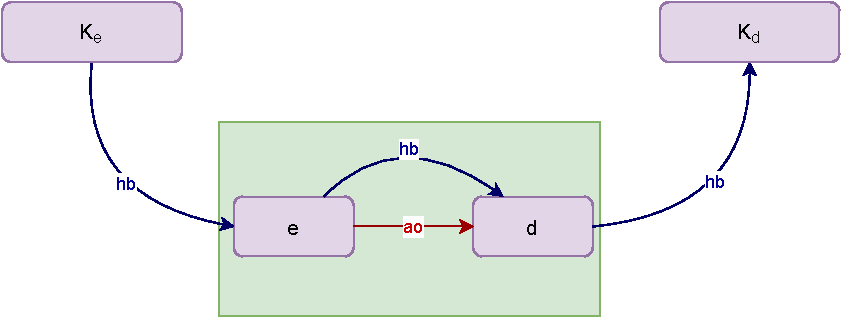
\includegraphics[scale=0.7]{Q1(a).pdf}
            \caption{For any Candidate Execution of $C$, the set $K_e$ and $K_d$}
            \label{fig:my_label}
        \end{figure}
        
        The idea is that if these relations are intact, then the relations among events from the first and second set will also hold due to transitivity.
        
        Consider two events $\event{p1}{K_e}$ and $\event{p2}{K_d}$ (When $e$ is the first event or $d$ is the last event, assume dummy events that can act as $p1$ or $p2$.) belonging to the same agent as that of $e$ and $d$ such that in $C$:
        \begin{align*}
            dir(p1,e)\ \wedge\ dir(d,p2).
        \end{align*}

        Note that in terms of direct happens-before relations, on reordering, any $Candidate Execution$ of $C$ will have the following changes
        
        %Show a figure here 
        \begin{figure}[H]
            \centering
            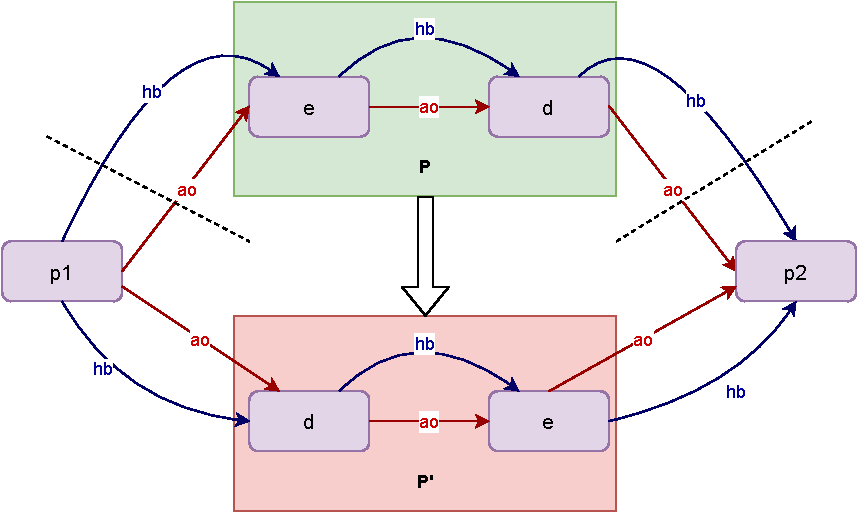
\includegraphics[scale=0.7]{Q1(b).pdf}
            \caption{The direct relation changes that can be observed while reordering events $e$ and $d$}
            \label{fig:my_label}
        \end{figure}
        
        The figure above is to show that, for any $Candidate Execution$ of $C$, the following is true
        \[
            cons(p1,e) \ \wedge dir(p1,e) \ \wedge dir(e,d) \ \wedge cons(d,p2) \ \wedge \ dir(d,p2).
        \]
        and for that of $C'$,
        \[
            cons(p1,d) \ \wedge \ dir(p1,d) \ \wedge \ dir(d,e) \ \wedge cons(e,p2) \ \wedge dir(e,p2).
        \]
        
        We need the following relations among $p1$, $p2$, $e$ and $d$ to be preserved in Candidate executions of $C'$ 
        \[
            \reln{p1}{hb}{e} \ \wedge \ \reln{p1}{hb}{d} \ \wedge \ \reln{d}{hb}{p2} \ \wedge \ \reln{e}{hb}{p2}.
        \]
        
        After reordering, we do have these relations preserved due to transitivity  
        \begin{gather*}
            \reln{p1}{hb}{d} \ \wedge \ \reln{d}{hb}{e} \ \Rightarrow \ \reln{p1}{hb}{e}. \\
            \reln{e}{hb}{p2} \ \wedge \ \reln{d}{hb}{e} \ \Rightarrow \ \reln{d}{hb}{p2}. \\
            \reln{p1}{hb}{d} \ \wedge \ \reln{d}{hb}{e} \ \wedge \ \reln{e}{hb}{p2} \ \Rightarrow \ \reln{p1}{hb}{p2}. 
        \end{gather*}
    
        If we can "pivot" the remaining set $K_e$ to $p1$ and $K_d$ to $p2$, it would ensure that our intended relations remain intact after reordering by transitivity. To state formally, we have a valid pair of pivots $<p1,p2>$ when the following two conditions hold
        \begin{gather*}
            \forall \ k \in K_e - \{p1\}, \ \reln{k}{hb}{p1}. \\
            \forall \ k \in K_d - \{p2\}, \ \reln{p2}{hb}{k}.
        \end{gather*}
        
        %Show a figure here
        \begin{figure}[H]
            \centering
            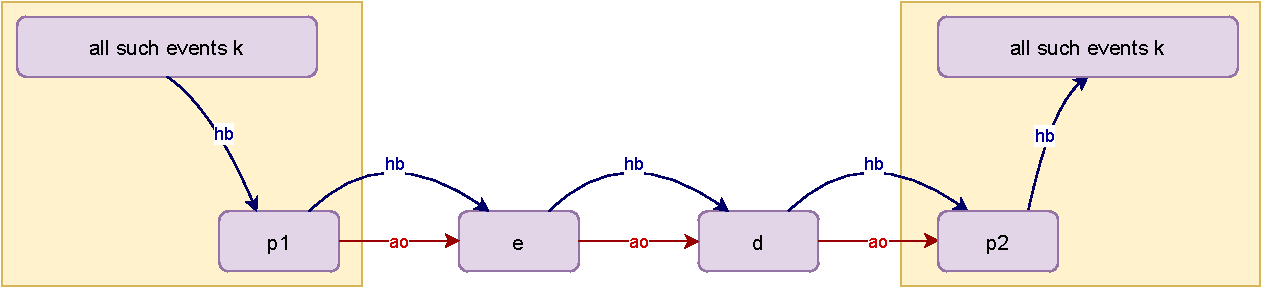
\includegraphics[scale=0.7]{Q1(d).pdf}
            \caption{For any Candidate execution, the intuition behind valid pivots $<p1,p2>$}
            \label{fig:my_label}
        \end{figure}
        
        By lemma 1 and lemma 2 respectively, we have for $C$, the following condition where $<p1, p2>$ is a valid pivot pair
        \begin{gather*}
            \et{e}{uo} \vee (\et{e}{sc} \wedge \event{e}{W}). \\
            \et{d}{uo} \vee (\et{d}{sc} \wedge \event{d}{R}).
        \end{gather*}
            
        The following table summarizes the cases where we have a valid pair of pivots $<p1,p2>$
        %Show a general table here 
        \begin{figure}[H]
            \centering
            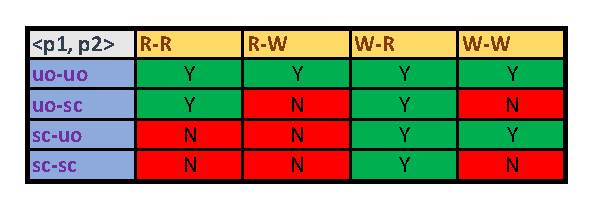
\includegraphics[scale=0.7]{Table1_Final.pdf}
            \caption{Table summarizing whether we have valid pair of pivots based on  $e$ and $d$}
            \label{fig:my_label}
        \end{figure}
                
        We show a simple example where we do not have a valid pair of pivots, particularly because $p1$ is not a valid pivot. Note that in this example, $K_e = K_{e1} + K_{e2} + p1 + p_x$
        %Show figure here of program P
        \begin{figure}[H]
            \centering
            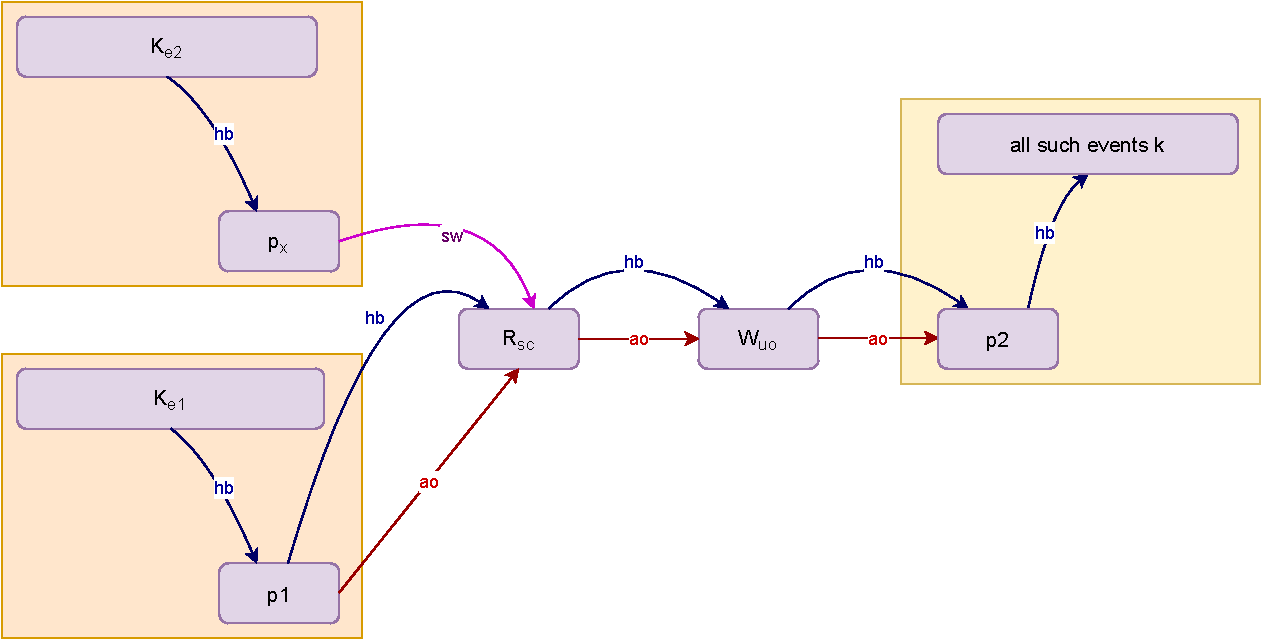
\includegraphics[scale=0.7]{Q1(e).pdf}
            \caption{A Candidate Execution where p1 is not a valid pivot}
            \label{fig:my_label}
        \end{figure}
        
        %Show figure here of program P'
         \begin{figure}[H]
            \centering
            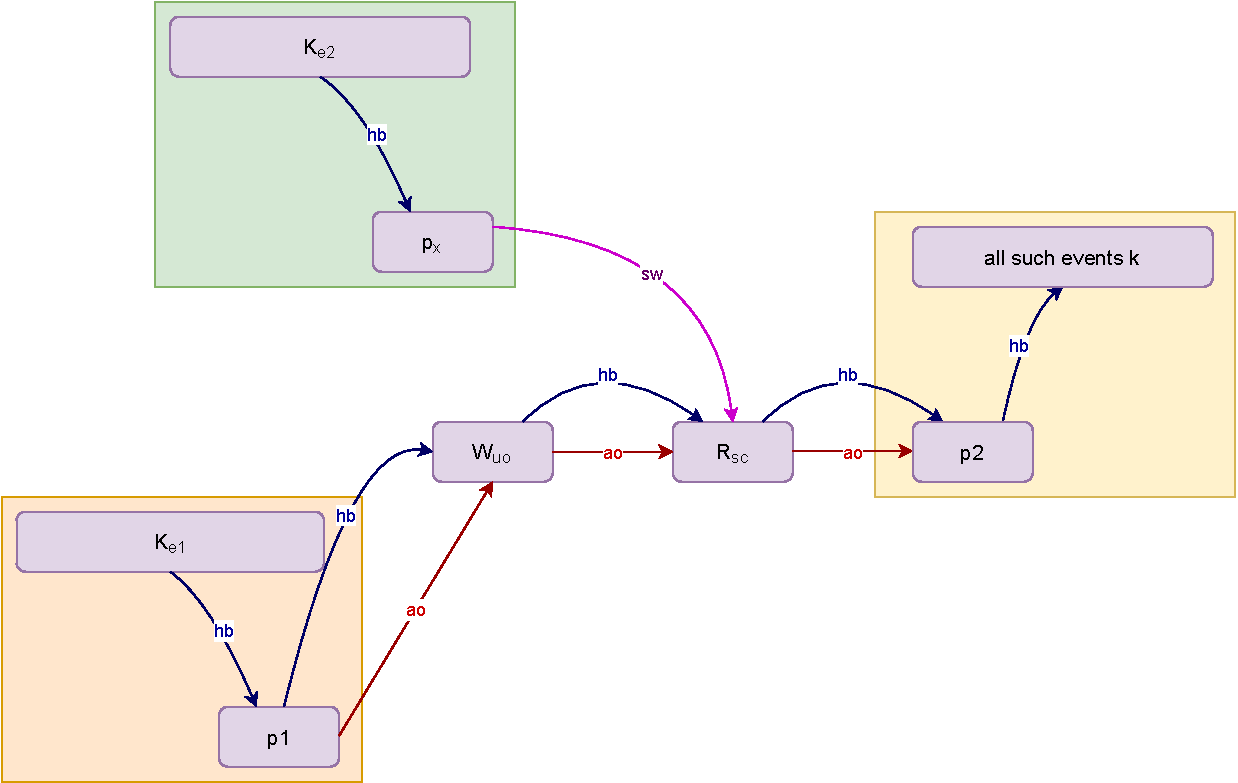
\includegraphics[scale=0.7]{Q1(f).pdf}
            \caption{The resultant Candidate Execution after reordering, exposing the relations with $p_x$, $K_{e2}$ and $d$ that are lost}
            \label{fig:my_label}
        \end{figure}
        
            
        %MAKE SOME MAJOR CHANGES TO THIS
        \paragraph{2. Additional \textit{happens-before} relations}
        Although we have identified the cases when \textit{happens-before} relations are preserved, we also get some additional relations in some of them.
        
        %Show an example here and explain
        As an example, for the case when $d$ is a sequentially consistent read, by lemma 1, in any execution of $C$
        \[
            \reln{k}{hb}{d} \centernot\Rightarrow \reln{k}{hb}{e} 
        \]

        But in $Executions$ of candidate $C'$, by transitivity, we have 
        \[
            \reln{k}{hb}{d} \Rightarrow \reln{k}{hb}{e} 
        \]
        
        This is because, there are sets of relations that come through certain \textit{synchronize-with} relations. Thus, although we are able to preserve relations that existed in any $Candidate Execution$ of $C$, we also in the process, introduce new ones in $Candidate Executions$ of $C'$. The figure below shows pictorially an example of a Candidate Execution of $C$ for the case above 
        
        %Show figure here of program P 
        \begin{figure}[H]
            \centering
            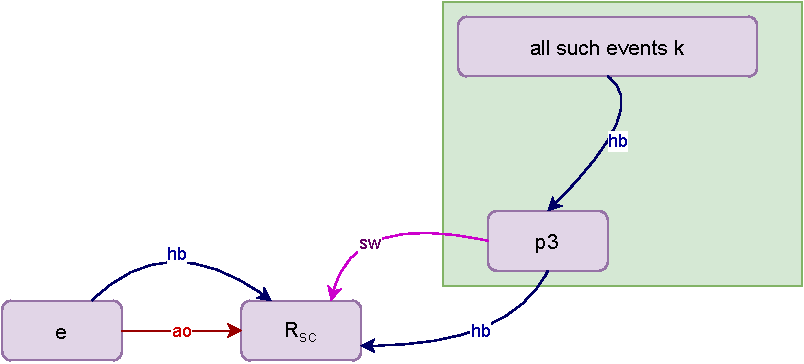
\includegraphics[scale=0.7]{Q2(c).pdf}
            \caption{A Candidate Execution where $d$ is a sequentially consistent read}
            \label{fig:my_label}
        \end{figure}
        
        %Show figure here of program P'
        \begin{figure}[H]
            \centering
            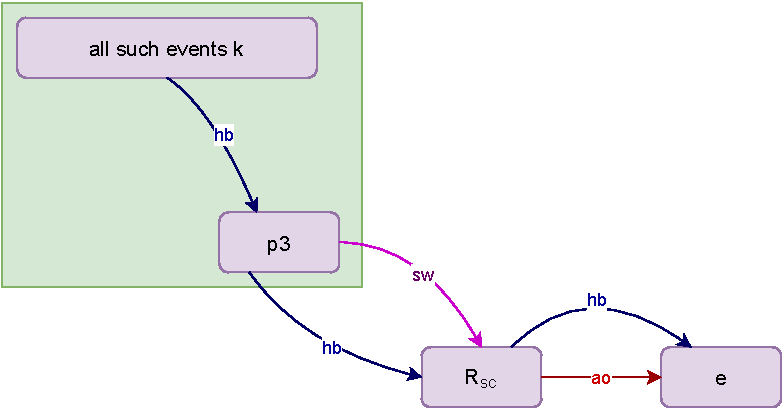
\includegraphics[scale=0.7]{Q2(d).pdf}
            \caption{The Candidate Execution after reordering, exposing the new relations established with $e$, $p3$ and set $k$}
            \label{fig:my_label}
        \end{figure}
        
        \critic{purple}{Explain the above figures or perhaps highlight the new relations that are established.}
       
       
        To summarize, the table below shows the cases where new relations could be introduced. 
        %Show the table here
        \begin{figure}[H]
            \centering
            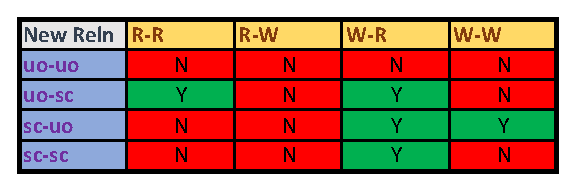
\includegraphics[scale=0.7]{Table2_Final.pdf}
            \caption{Table summarizing when new \textit{happens-before} relations could be introduced based on having valid pair of pivots }
            \label{fig:my_label}
        \end{figure}

        For these cases, we must know whether these new relations introduce new observable behaviors. 
        
%--------------------------------------------------------------------------------------------------------------------------------------
    \paragraph{4. Presence of cycles?}
        Before we go into analyzing whether new relations introduce observable behaviours, we first ensure there are no $\stck{_\textit{hb}}$ cycles introduced in the process. Consider the example below
        \begin{figure}[H]
            \centering
            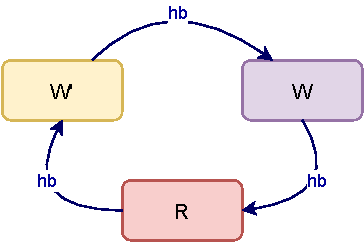
\includegraphics[scale=0.7]{Q4(a).pdf}
            \caption{Caption}
            \label{fig:my_label}
        \end{figure}
        
        Notice that here, the axiom of coherent reads restricts $R$ to read from $W'$.
        \[
            \reln{R}{hb}{W'} \Rightarrow \neg \reln{R}{rf}{W'}
        \]
        
        But by transitive property, it is also the case that $\reln{W'}{hb}{R}$. 
        \[
            \reln{W'}{hb}{W} \ \wedge \ \reln{W}{hb}{R} \ 
            \Rightarrow \ 
            \reln{W'}{hb}{R}
        \]
        
        As per this, the axiom of coherent reads shouldn't restrict $\reln{R}{rf}{W'}$. To avoid such cases, we will need to ensure that no Candidate Execution of $C'$ after $e$ and $d$ are reordered have $\stck{_{hb}}$ cycles.
        
        Note that if a cycle exists after reordering, then 
        \begin{enumerate}
            \item The relations preserved do not themselves create a cycle (ref to the theorem)
            \item Additional new relations may introduce cycles
        \end{enumerate}
       
        The first part is straightforward as we assume we can only do reordering on Candidate Exectuions of $C$ not having cycles. 
        
        To address the second part, we first address the cases where $\reln{d}{hb}{e}$ may be part of the cycle. The other event $k$, may be either from the set $K_e$, $K_d$ or a new relation that is formed.
        %Show figure here
        \begin{figure}[H]
            \centering
            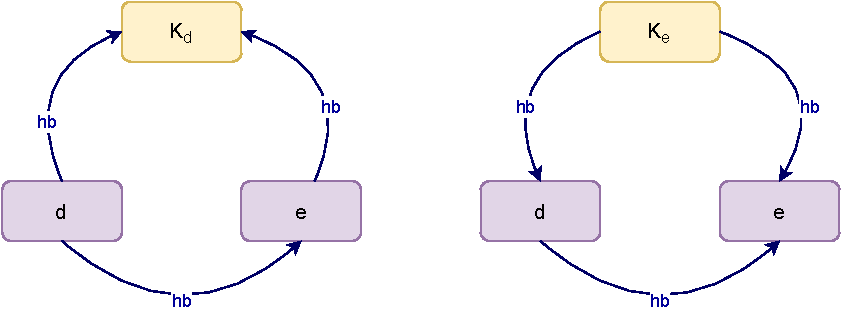
\includegraphics[scale=0.7]{Q4(a)_1.pdf}
            \caption{If k belongs to one of the sets $K_e$ or $K_d$}
            \label{fig:my_label}
        \end{figure}
        
        The above figure shows that $k$ cannot belong to either of the sets, as their relations with $e$ and $d$ will not result in a cycle. 
        
        For cases where $\reln{k}{hb}{e}$ is the set of new relations, note that by lemma 1
        \[
            \reln{k}{hb}{e} \Rightarrow \reln{k}{hb}{d}
        \]
        
        For cases where $\reln{d}{hb}{k}$ is the set of new relations, by lemma 2
        \[
            \reln{d}{hb}{k} \Rightarrow \reln{e}{hb}{k}
        \]
        
        So for both these cases also, a cycle with $\reln{d}{hb}{e}$ cannot exist. The following figure shows pictorially this fact. 
        %Show figure here
        \begin{figure}[H]
            \centering
            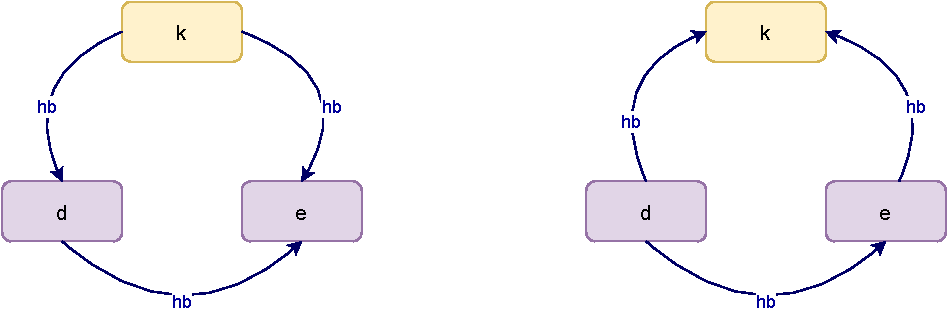
\includegraphics[scale=0.7]{Q4(a)_2.pdf}
            \caption{If $\reln{k}{hb}{e}$ or $\reln{d}{hb}{k}$ are new sets of relations}
            \label{fig:my_label}
        \end{figure}
        
        
        For the one case where we have two new sets of relations formed, i.e $\reln{d}{hb}{k}$ and $\reln{k}{hb}{e}$, we could have a case where $k$ is a common event for both sets. But, by lemma 1, we also have $\reln{k}{hb}{d}$ and by lemma 2, $\reln{e}{hb}{k}$. Thus, we have a cycle. The following figure shows this pictorially
        
        %Show figure here
        \begin{figure}[H]
            \centering
            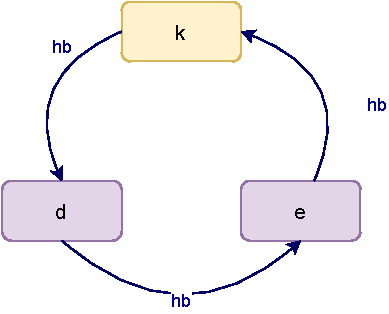
\includegraphics[scale=0.7]{Q4(a)_3.pdf}
            \caption{A cycle exists in the case where we have two new sets of relations ($\reln{k}{hb}{e}$ and $\reln{d}{hb}{k}$) }
            \label{fig:my_label}
        \end{figure}
        
        \critic{purple}{Maybe have a better figure, meaning a set of relations where each figure shows clearly which relaiton is implied due to whcih lemma}

        Now for the case when $\reln{d}{hb}{e}$ may not be part of the cycle, we have only two other relations, $\reln{k}{hb}{e}$ or $\reln{d}{hb}{k}$.
        
        Considering the first scenario where the new set of relations are of the form $\reln{k}{hb}{e}$. Suppose a cycle exists with another event $k'$. Then 
        \[
            \reln{k}{hb}{e} \ \wedge \
            \reln{e}{hb}{k'} \ \wedge \
            \reln{k'}{hb}{k}
        \]
        
        Note that the latter two relations are not new, since the only new set of relations are of the first form. Now, by lemma 1 and by transitivity respectively
        \begin{gather*}
            \reln{k}{hb}{e} \Rightarrow \reln{k}{hb}{d} \\
            \reln{e}{hb}{k'} \Rightarrow \reln{d}{hb}{k'}    
        \end{gather*}
        
        So, the following is also a cycle
        \[
            \reln{k}{hb}{d} \ \wedge \
            \reln{d}{hb}{k'} \ \wedge \
            \reln{k'}{hb}{k}
        \]
        
        But these relations already exist in the original Candidate Execution, which implies a cycle existed before reordering. This contradicts our assumption that we only reorder when the Candidate Executions of $C$ have no cycles. Thus, by contradiction such a cycle cannot exist.
        
        In similar lines for the cases where the set of new relations are of the form $\reln{d}{hb}{k}$, we can show by contradiction that a cycle cannot exist.

%-------------------------------------------------------------------------------------------------------------------------------------

        %Needs a few major changes and tables split cases into disjoint, overlapping and equal ranged events 
        \paragraph{4. Do new relations introduce new observable behaviors?}
        In any candidate execution, reordering events $e$ and $d$ eliminates the relation $\reln{e}{hb}{d}$ and introduces the new relation $\reln{d}{hb}{e}$. 
        New behaviours created by the latter directly, if any, are 
        of course intentional (and should normally be avoided by ensuring $e$ and $d$ are independent), but we need to ensure that this does not also result in new behaviours indirectly. 
        
        On observing the role on the axioms on this relation, notice that if both $e$ and $d$ are read events then the range does not matter. For all other cases, if events $e$ and $d$ have overlapping ranges, one could introduce a new observable behavior after reordering them (a simple use of Coherent Reads / Sequentially Consistent Atomics).     
        
        Any other new relations that are introduced can be divided into 4 cases, in terms of our events $e$ and $d$ and the new relation with some event $k$:
        %Show a figure here summarizing the four cases
        \begin{figure}[H]
            \centering
            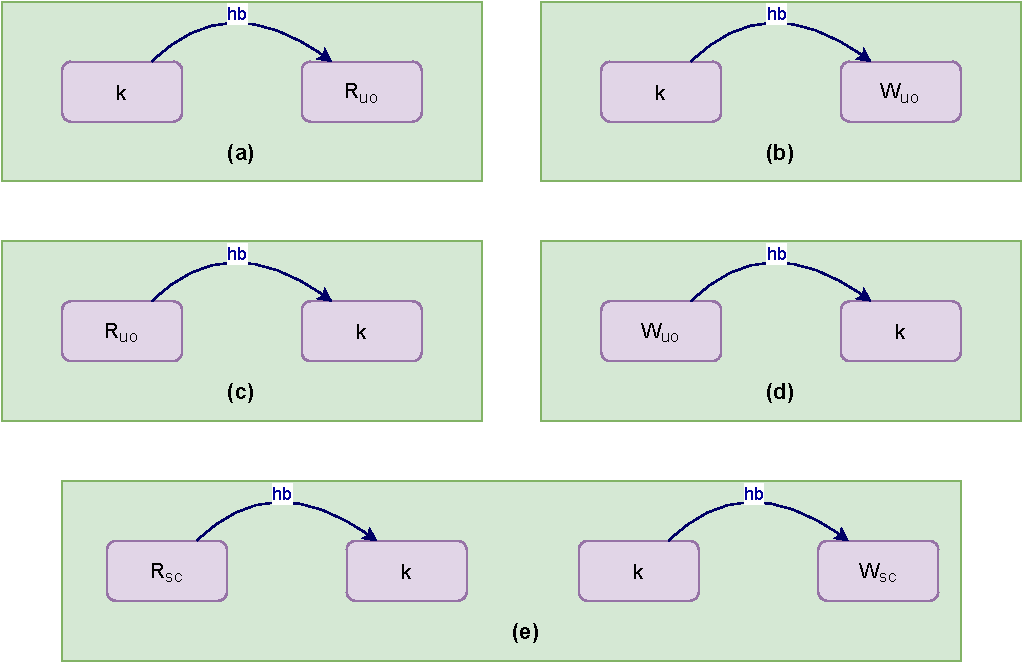
\includegraphics[scale=0.7]{Q3(a).pdf}
            \caption{Caption}
            \label{fig:my_label}
        \end{figure}
        
        \critic{purple}{Change the figure above to represent only the first four cases}

        In each of the above cases, note firstly that we need to only consider cases where their ranges are overlapping/equal.
        
        %Addressing the first case. 
        Figure below shows a breakdown of sub-cases for the first case (a), varying based
        on the nature of event $k$.
        %Show all cases here for different k
        \begin{figure}[H]
            \centering
            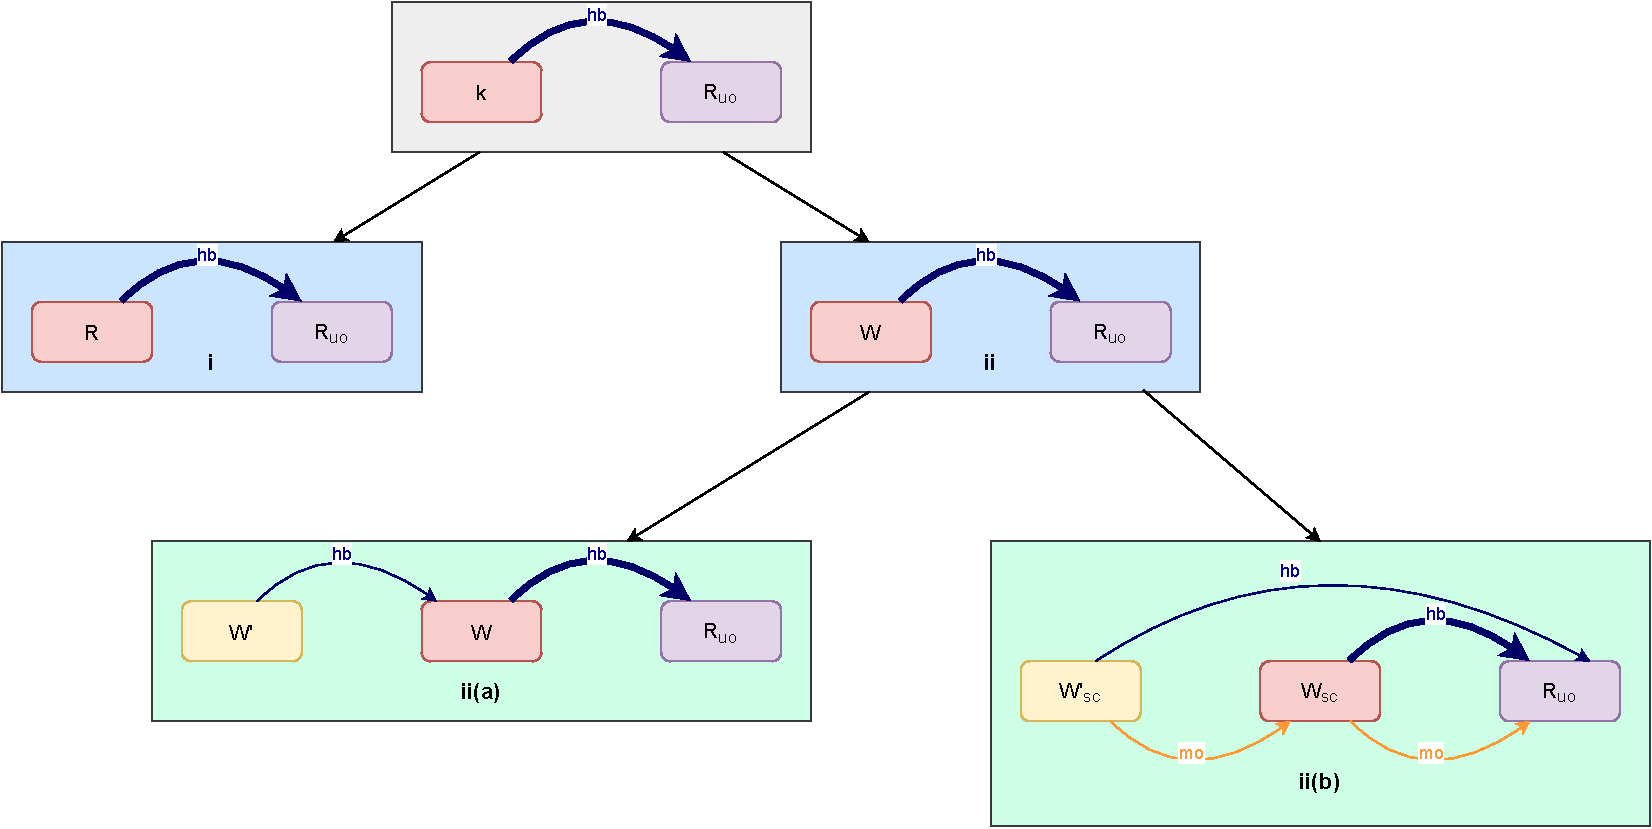
\includegraphics[scale=0.6]{Q3_(b)Case1.pdf}
            \caption{The role of the axioms on introducing a new relation between an unordered Read and some event $k$}
            \label{fig:my_label}
        \end{figure}
        
        %Might have to elaborate this more
        \begin{enumerate}
            \item For (i), when $k$ is a read, none of the rules have any implications on observable behaviors.
            \item For (ii), when $k$ is a write, the rule of coherent reads (ii(a)) or sequentially consistent atomics (ii(b)) could restrict the read ($e$) from reading overlapping ranges of $W'$ with $W$.
        \end{enumerate}
        
        The above case analysis shows us that the new relation could 'trigger' the consistency rules, only to restrict possible reads-from relations, thus restricting possible observable behaviors. 

        The other cases, also have instances which can 'trigger' some cases of the axioms, thus restricting possibly some $\stck{_{rf}}$ relations.b These cases are shown in the figures below: 
        \begin{figure}[H]
            \centering
            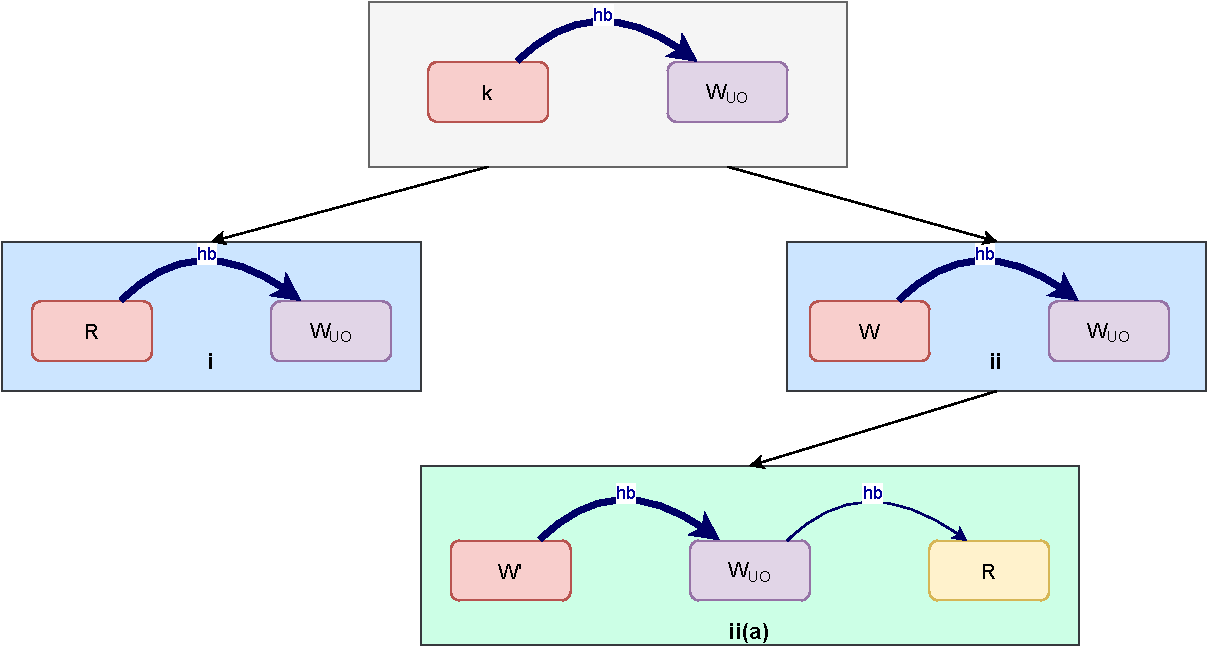
\includegraphics[scale=0.6]{Q3_(c)Case2.pdf}
            \caption{(i) and (ii(b)) satisfy the axiom of Coherent Reads}
            \label{fig:my_label}
        \end{figure}
              
        \begin{figure}[H]
            \centering
            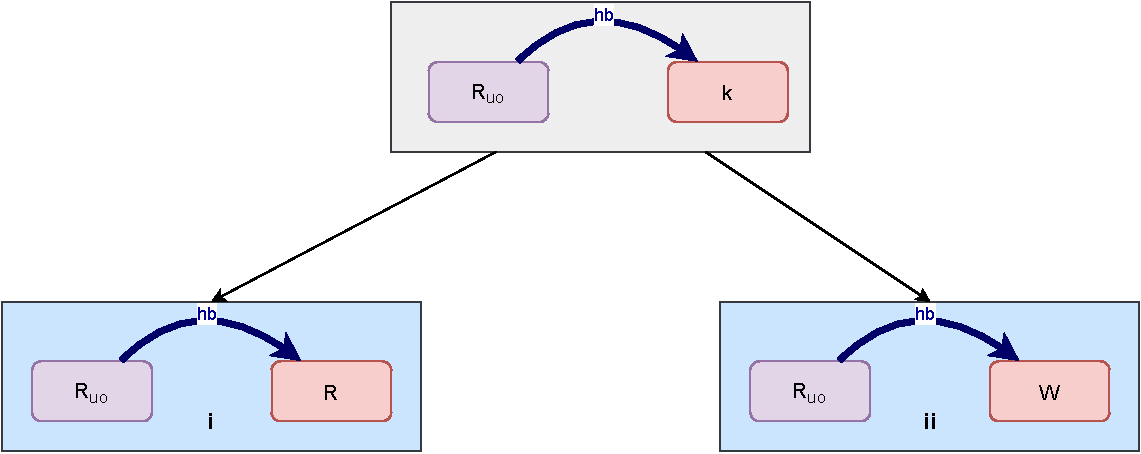
\includegraphics[scale=0.6]{Q3_(d)Case3.pdf}
            \caption{(ii) satisfies the axiom of Coherent Reads}
            \label{fig:my_label}
        \end{figure}
        
        \begin{figure}[H]
            \centering
            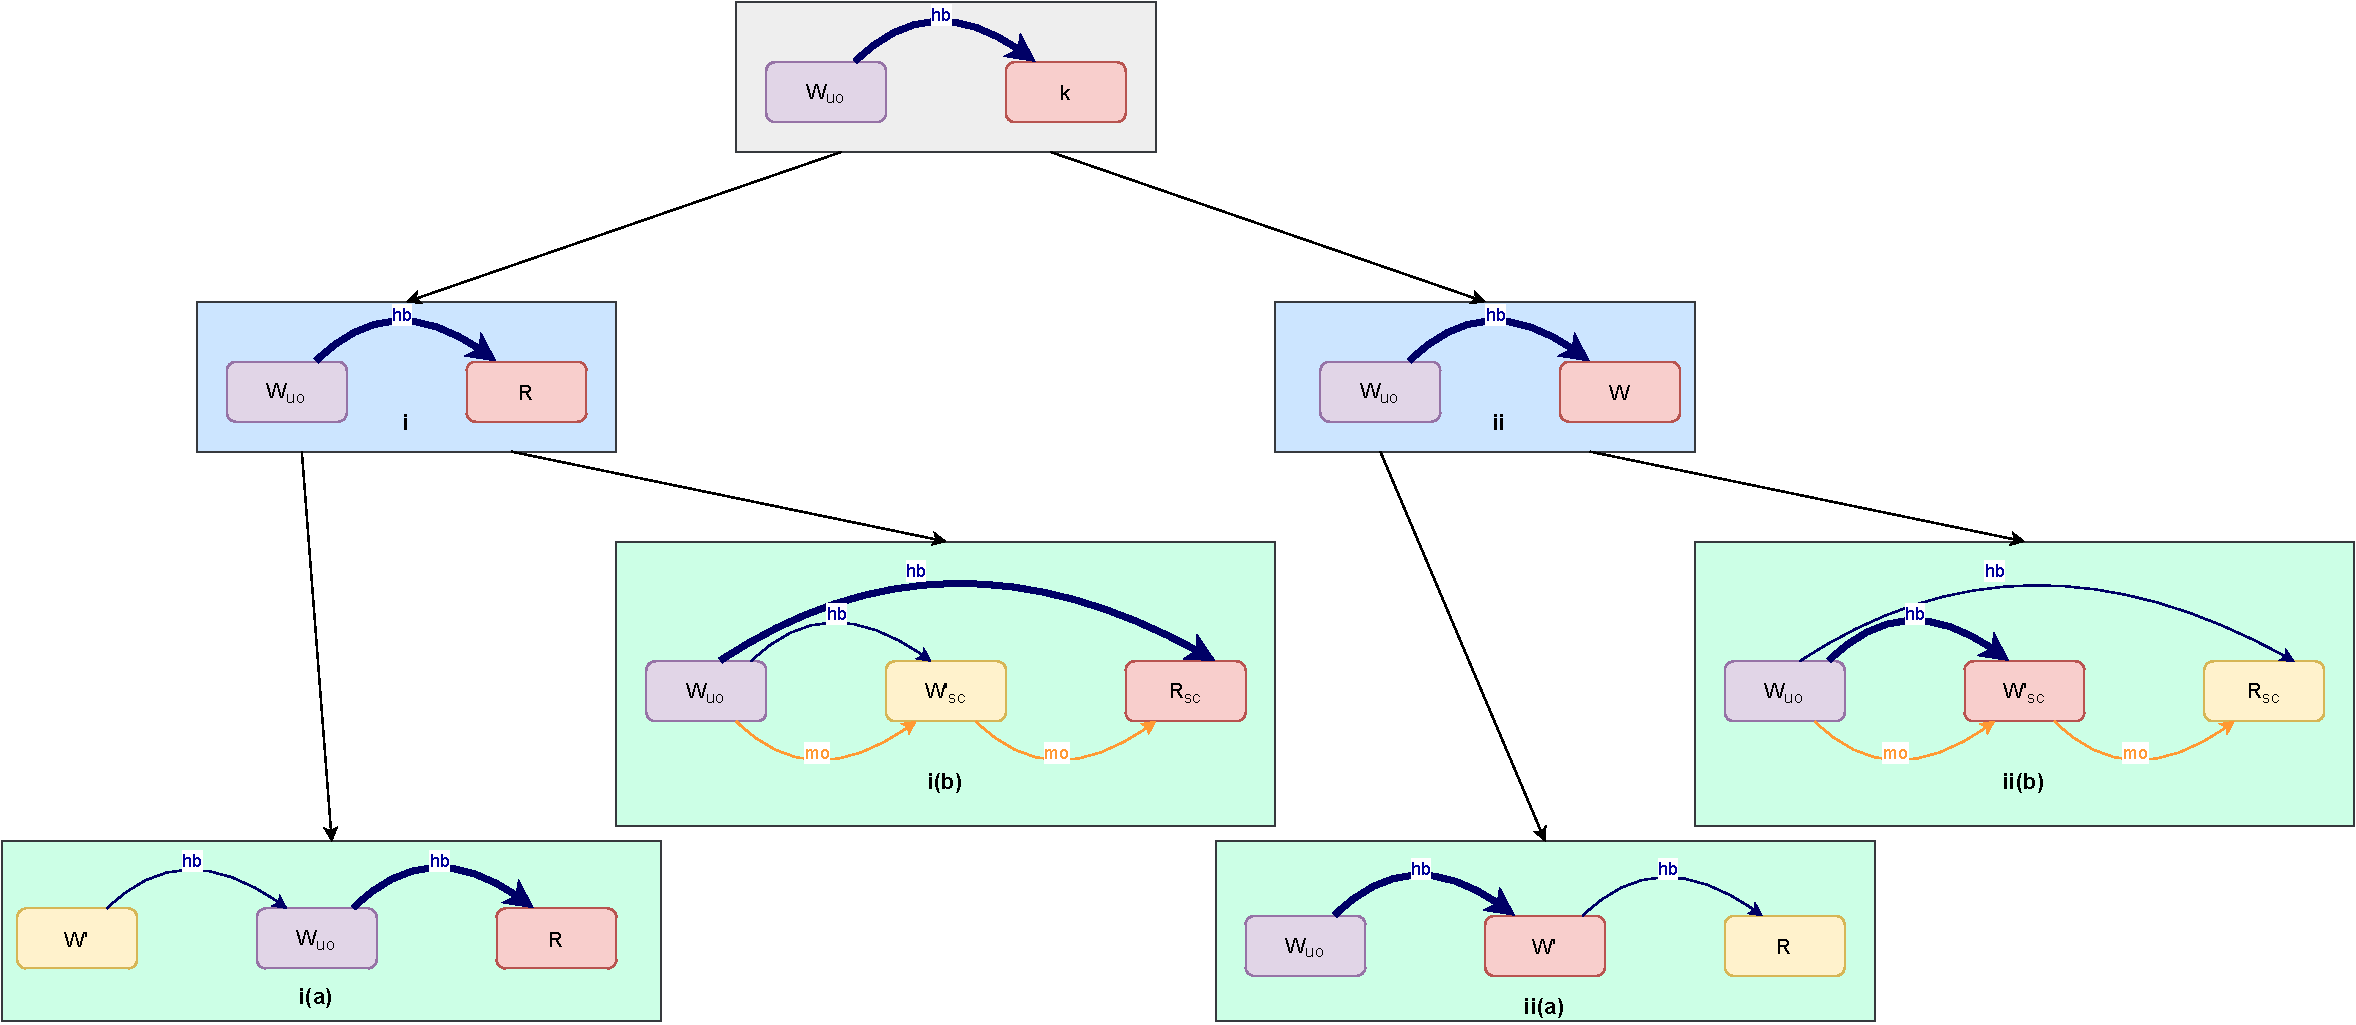
\includegraphics[scale=0.4]{Q3_(e)Case4.pdf}
            \caption{(i(a)), (ii(a)) satisfy the axiom of Coherent Reads, whereas (i(b)), (ii(b)) satisfy the axiom of Sequentially Consistent Atomics}
            \label{fig:my_label}
        \end{figure}
        
        \critic{blue}{The main reason for this is that we framed he axioms in a form that restricts \textit{reads-from} relations. So in any case where adding an additional \textit{happens-before} relation "triggers" an axiom, we are bound to have some behaviors restricted. It is this fact that is elicited explicitly by going case wise on all relations that are introduced.}
     
        The table below summarizes the valid cases where, we have a pair of valid pivots, where new relations do not introduce new observable behaviors and do not have cycles. 
        %Show the table here
        \begin{figure}[H]
            \centering
            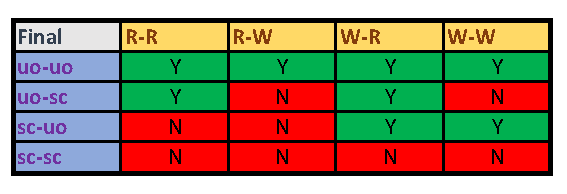
\includegraphics[scale=0.7]{Table4_Final.pdf}
            \caption{The final table summarizing the valid cases where observable behaviors will only be a subset after reordering.}
            \label{fig:my_label}
        \end{figure}

        \critic{blue}{Keep in mind that the comparision of ranges is done while addressing question 3 in the proof, so the table above, implicitly also takes into account only the valid cases where ranges are also correct}
    
        The table above, precisely is the definition of a reorderable pair. If we write the above table in the form of an expression we have an expanded format of our Reorderable pair function. 

        \begin{align*}
            Reord(e,d) = \\
            (
            ((\et{e}{uo} \wedge \et{d}{uo}) \ \wedge \\ 
                \quad ( 
                        &(\event{e}{R} \wedge \event{d}{R}) \vee \\ 
                        &(\event{e}{W} \wedge \event{d}{R} \wedge (\Re(e) \And \Re(d) = \phi)) \vee \\
                        &(\event{e}{R} \wedge \event{d}{W} \wedge (\Re(e) \And \Re(d) = \phi)) \vee \\
                        &(\event{e}{W} \wedge \event{d}{W} \wedge (\Re(e) \And \Re(d) = \phi)) 
                    )
            ) \\ \vee \\
            ((\et{e}{sc} \wedge \et{d}{uo}) \ \wedge \\
                \quad (
                        & (\event{e}{W} \wedge \event{d}{R} \wedge (\Re(e) \And \Re(d) = \phi)) \vee \\
                        & (\event{e}{W} \wedge \event{d}{W} \wedge (\Re(e) \And \Re(d) = \phi)) 
                    )
            ) \\ \vee \\
            ((\et{e}{uo} \wedge \et{d}{sc}) \ \wedge \\
                \quad (
                        & (\event{e}{R} \wedge \event{d}{R} \wedge) \vee \\
                        & (\event{e}{W} \wedge \event{d}{R} \wedge (\Re(e) \And \Re(d) = \phi)) 
                    )
            )
            )
        \end{align*}
        
        \qed  
\end{proof}

\begin{corollary}
    Consider a Candidate C of a program and its Candidate Executions which are valid. Consider two events $e$ and $d$ such that $\neg \cons{e}{d}$ is true in C and $\reln{e}{ao}{d}$. Consider another Candidate C' resulting after reordering $e$ and $d$ in C. Then, the set of Observable behaviors possible in C' is a subset of C only if $Reord(e,d)$ and the following holds true.
    
    \[
        \forall \ k \ \textit{s.t.} \ 
        \reln{e}{ao}{k} \ \wedge \ \reln{k}{ao}{d} \ . \ 
        Reord(e,k) \ \wedge \ Reord(k,d)
    \]
    
\end{corollary}
    
\begin{proof}
    
\end{proof}
    
\subsection{Counter examples for the invalid cases}

\subsection{}

    

    
    
    
    
    